\DailyTitle{6332 Log (October 26, 2010)}

\DailySection{Goals}

\begin{enumerate}
\item Make a plan for Hcal sample rerunning.
\item Finish up vecbos note - aim for Thursday, first draft
\item Make a plan for noiseline deployment
\end{enumerate}

\DailySection{Summary List}

\begin{enumerate}
\item The duplicate-checking jobs are done.  Lots of duplicate events found.  Some missing files spotted.
\item Added ieta-iphi plots to Hcal DQM testbench for the two discriminators.  {\bf Linear double-chi2 picks out the famous (14, 31) cell.}
See plot \ref{Figure_6332DQMFamousCellLambdaLinear}.
\item Made a short noise DQM presentation at the group meeting.
\end{enumerate}

\begin{figure}
   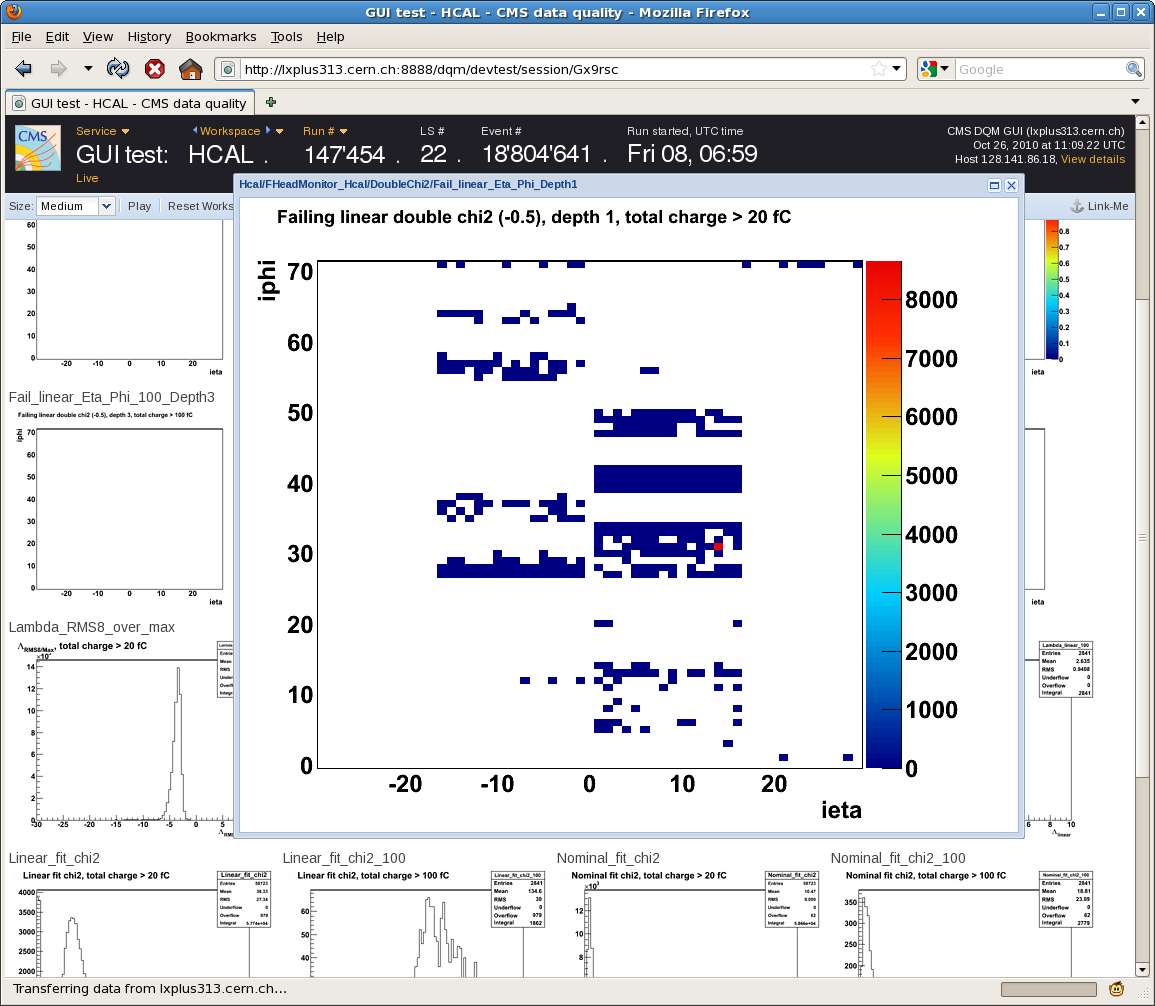
\includegraphics[width=120mm]{DailyLog/6332/6332Kerker.png}
   \caption{Linear double chi2 picks out the famous hot cell}
   \label{Figure_6332DQMFamousCellLambdaLinear}
\end{figure}

\DailySection{Planning for Hcal noise studies}

Things I need to check:

\begin{enumerate}
\item Different total charge threshold?
\item Event cleaning.  What to use for the ``cleaning'' of noise sample.
\item Check on MC pulse shape.
\item Correlation with other rechit filters.  How?
\item Other subtypes of noise?
\item Check signal distribution channel by channel.
\item Run on different types of runs.
\item Geometrical locations of each type of noise.
\item Look at observables, ex. MET distribution in signal events.
\item (Education purpose)  Figure out how to estimate ratiation level.
\end{enumerate}

\DailySection{Hcal noise double-chi2: total charge threshold}

The relative number of cells that will be included with different total charge threshold cut is shown in table \ref{Table_6332RelativePulseCountTotalChargeThreshold}.
The ntuple size for run 135175 (20fC threshold) signal is 637MB, and for noise it is 230MB.  The total size is then 867MB.
If we go to 10 fC threshold, it will be roughly 3GB.  Let's now say that the size of dataset grows linearly with luminosity (worst case scenario).
The integrated luminosity of run 135175 is 0.4/nb, so it will be 7.5GB per inverse nb, 7.5TB per inverse pb.
So....O(TB) space needed.  Still okay.

Interesting note: for pulses that are too small, signal hypothesis will always work better than linear or RMS/Max, in the presense of pedestal fluctuation.
For pulses within 1-5 fC, this is always true.  10-20 fC, a little bit of discrimination power remains.  In other words, 10fC is a good threshold for now.

\begin{table}
   \centering
   \begin{tabular}{|c|c|c|c|c|c|c||c|c|}
      \hline
      Threshold (fC) & 1 & 3 & 5 & 10 & 20 & 100 & 1-5 & 10-20 \\\hline
      Number of pulses & 2736251 & 720865 & 276245 & 94951 & 27272 & 1307 & 2460006 & 67679 \\\hline
      Rough ratio to next & 3.8x & 2.6x & 2.9x & 3.5x & 20.9x & N/A & N/A & N/A \\\hline
   \end{tabular}
   \caption{Relative number of pulses for different total charge threshold cut}
   \label{Table_6332RelativePulseCountTotalChargeThreshold}
\end{table}

